\ylDisplay
{}% Problem name
{2021}% Year
{mcq}% Round (mcq, theory, experiment)
{1}% Problem nr.
{physics}% Subject (physics, chemistry, biology)
{}% Difficulty (1-3)
{
% Syl:
\ifStatement
A stationery siren goes on at a constant frequency in front of (outside) a merry-go-round. If the merry-go-round is rotating in the clockwise direction with the siren as shown in the figure. Following are some conditions at which higher frequency, lower frequency, and the original frequency are observed by a person sitting on the merry-go-round.
\begin{center}
  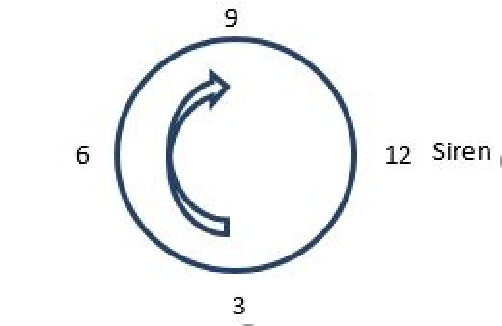
\includegraphics[width=0.4\linewidth]{2021-mcq-01-p}
\end{center}
Select the correct statements from the following four options.
\begin{enumerate}
  \item Original pitch is heard at 12 O’clock and 6 O’clock positions.
  \item Original pitch is heard at 9 O’clock and 3 O’clock positions.
  \item Higher pitch is heard at 3 O’clock and lower pitch at 9 O’clock positions.
  \item Higher pitch is heard at 9 O’clock and lower pitch at 3 O’clock positions.
\end{enumerate}
\fi


\ifOption1
1 and 4
\fi


\ifOption2
2 and 3
\fi


\ifOption3
1 and 3
\fi


\ifOption4
2 and 4
\fi


\ifHint

\fi


\ifSolution

\fi


\ifEstStatement
% Problem name:

\fi


\ifEstOption1

\fi


\ifEstOption2

\fi


\ifEstOption3

\fi


\ifEstOption4

\fi


\ifEstHint

\fi


\ifEstSolution

\fi
}
